
%(BEGIN_QUESTION)
% Copyright 2010, Tony R. Kuphaldt, released under the Creative Commons Attribution License (v 1.0)
% This means you may do almost anything with this work of mine, so long as you give me proper credit

Examine this control circuit diagram for an air compressor, where a pair of pressure switches controls the starting and stopping of the electric motor turning the air compressor:

$$\includegraphics[width=15.5cm]{i04056x01.eps}$$

Explain what the ``Hand-Off-Auto'' switch does in this circuit, and also describe the functions of each pressure switch.

\vskip 20pt \vbox{\hrule \hbox{\strut \vrule{} {\bf Suggestions for Socratic discussion} \vrule} \hrule}

\begin{itemize}
\item{} Which of these two pressure switches should have the greater trip setting, and why?
\item{} Why do you think operations personnel might find it useful to have a ``Hand'' position as well as an ``Auto'' position on the switch in this air compressor system?
\item{} Some ``Hand-Off-Auto'' switches place the ``Auto'' position in the middle, between the ``Hand'' and the ``Off'' settings -- explain why this might be a better way to arrange the three-position switch.
\item{} Identify the consequences of jumpering across the OL switch contacts in this circuit using a piece of wire.
\item{} Identify the consequences of jumpering across the Cut-out pressure switch contacts in this circuit using a piece of wire.
\item{} Identify the consequences of jumpering across the ``M'' contactor coil in this circuit using a piece of wire.
\item{} Identify the consequences of jumpering across the Control pressure switch contacts in this circuit using a piece of wire.
\item{} Identify the consequences of jumpering across the ``M'' contactor coil in this circuit using a piece of wire.
\item{} Identify the consequences of jumpering between the ``Hand'' and ``Auto'' terminals on the manual selector switch using a piece of wire.
\end{itemize}

\underbar{file i04056}
%(END_QUESTION)





%(BEGIN_ANSWER)


%(END_ANSWER)





%(BEGIN_NOTES)

In the ``hand'' position, the control switch is bypassed, allowing the compressor to run and raise pressure past the control switch's trip setting.  In the ``off'' position, the compressor is forced to turn off no matter what the status of either switch.  In the ``auto'' position, the compressor will be controlled by the status of the control switch: turning on when pressure is below that switch's trip point, and turning off when pressure is above the trip point.

\vskip 10pt

The function of the cut-out switch -- which is never bypassed -- is to protect the compressor from over-pressuring in the event the control switch fails closed.


\vskip 20pt \vbox{\hrule \hbox{\strut \vrule{} {\bf Virtual Troubleshooting} \vrule} \hrule}

This question is a good candidate for a ``Virtual Troubleshooting'' exercise.  Presenting the diagram to students, you first imagine in your own mind a particular fault in the system.  Then, you present one or more symptoms of that fault (something noticeable by an operator or other user of the system).  Students then propose various diagnostic tests to perform on this system to identify the nature and location of the fault, as though they were technicians trying to troubleshoot the problem.  Your job is to tell them what the result(s) would be for each of the proposed diagnostic tests, documenting those results where all the students can see.

During and after the exercise, it is good to ask students follow-up questions such as:

\begin{itemize}
\item{} What does the result of the last diagnostic test tell you about the fault?
\item{} Suppose the results of the last diagnostic test were different.  What then would that result tell you about the fault?
\item{} Is the last diagnostic test the best one we could do?
\item{} What would be the ideal order of tests, to diagnose the problem in as few steps as possible?
\end{itemize}


\vfil \eject

\noindent
{\bf Prep Quiz:}

The ``Hand'' position on a {\it Hand-Off-Auto} switch performs what function in a motor control system?

\begin{itemize}
\item{} Locks out power to the motor, so it is safe for people to work on
\vskip 5pt 
\item{} Forces the motor to shut off, no matter what else may be happening
\vskip 5pt 
\item{} Resets the thermal overload contact, to enable the motor to re-start
\vskip 5pt 
\item{} Allows the motor to turn on and off on its own, according to process needs
\vskip 5pt 
\item{} Mechanically locks the motor shaft so it cannot turn even if forced by hand
\vskip 5pt 
\item{} Forces the motor to turn on, even if auto mode operation would have it stop
\end{itemize}

\vfil \eject

\noindent
{\bf Prep Quiz:}

The ``Auto'' position on a {\it Hand-Off-Auto} switch performs what function in a motor control system?

\begin{itemize}
\item{} Locks out power to the motor, so it is safe for people to work on
\vskip 5pt 
\item{} Forces the motor to shut off, no matter what else may be happening
\vskip 5pt 
\item{} Resets the thermal overload contact, to enable the motor to re-start
\vskip 5pt 
\item{} Allows the motor to turn on and off on its own, according to process needs
\vskip 5pt 
\item{} Mechanically locks the motor shaft so it cannot turn even if forced by hand
\vskip 5pt 
\item{} Forces the motor to turn on, even if auto mode operation would have it stop
\end{itemize}

%INDEX% Electronics review: AC motor control circuit
%INDEX% Process: air compressor and receiver tank

%(END_NOTES)

